\documentclass[../main.tex]{subfiles}

\begin{document}

\subsubsection*{Methodology}
\subsubsection*{Data analysis}

    \begin{figure}
        \centering
        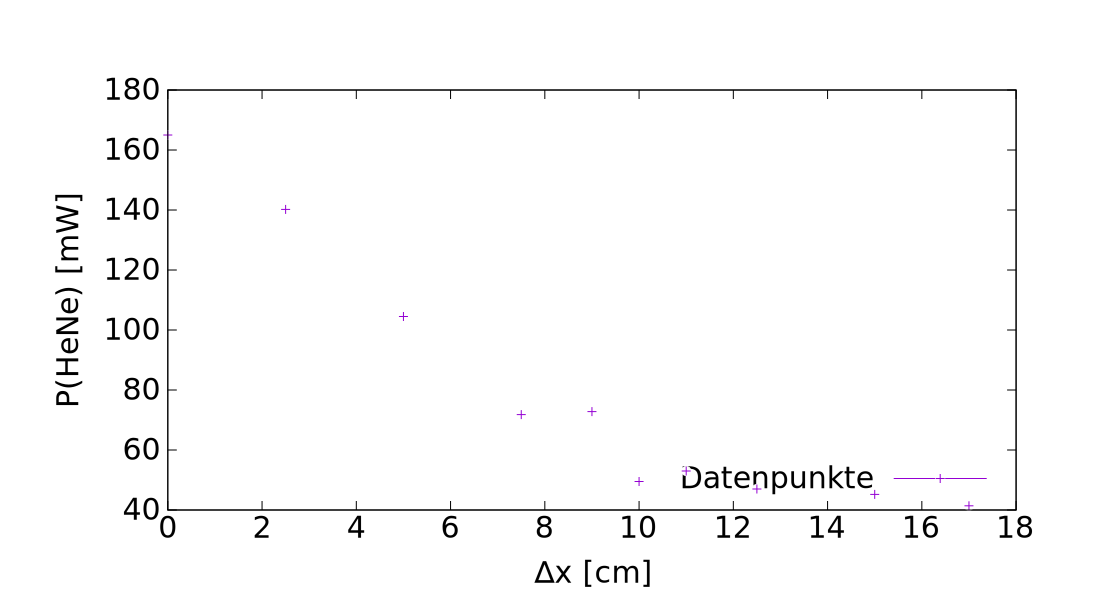
\includegraphics[width=0.8\textwidth]{Bilddateien/3/P(HeNe)overDx.png}
        \caption{The output power of the HeNe laser as a function of the displacement of the active medium, starting at $L_0:=\SI{35.5(1)}{\cm}$ on the given scale.}
        \label{fig:output_power_over_displacement}
    \end{figure}

    Looking at figure \ref{fig:output_power_over_displacement} we can see a linear dependency in the beginning inteval $[2,10]$. The fast decline in lasing power could be explained by the defocused reflextion beams inside the resonator, which was curved at one end and linear at the other, from which we deplaced the medium in the experiment. Therefore the effective beam cross-section decreases and the possibility of stimulated emission decreases with it.

\end{document}